\section*{Lời nói đầu}
C++ Standard Template Library (Thư viện STL) là một tập hợp các lớp dựng sẵn, cung cấp các cấu trúc dữ liệu phổ biến trong lập trình như: list, array, stack, queue, ... và các hàm phục vụ cho các cấu trúc dữ liệu đó, cũng như các thuật toán thông dụng.\\
Nhận thấy thư viện STL là một chủ đề thú vị, giúp ích cho các lập trình viên cho quá trình lập trình nói chung và lập trình hướng đối tượng nói riêng, nhóm chúng em quyết định chọn đây là đề tài tìm hiểu cho chuyên đề môn học Phương pháp lập trình hướng đối tượng.\\

\newpage
\tableofcontents
\listoffigures
%\listoftables

\newpage
\section{Tổng quan về STL}
Thư viện STL là một thư viện cung cấp các "khuôn mẫu" (template) cho các cấu trúc dữ liệu, cung cấp các thuật toán liên quan.\\
Thư viện STL có $4$ "thành phần" (components) chính: \cite{general}
\begin{itemize}
    \item Thuật toắn (algorithms): gồm các thuật toán được xây dựng chủ yếu cho các cấu trúc dữ liệu, ví dụ như: sort, search, ..
    \item Containers: chủ yếu gồm các cấu trúc dữ liệu thông dụng.
    \item Các hàm (functions): thư viện STL chứa các class có chứa toán tử được nạp chồng ("overload the function call operator"). Các class như vậy được gọi là "function objects" hoặc "functors".
    \item Iterators: iterators thường được dùng để xử lý một dãy các giá trị.
\end{itemize}
Theo như thỏa thuận giữa hai nhóm cùng làm chuyên đề \textit{Thư viện STL}, nhóm chúng em sẽ trình bày về \textbf{containers} và \textbf{iterators}.

\section{Các khái niệm}
\subsection{Iterators}
Trong C++, iterator (tạm dịch: biến lặp) là đối tượng bất kỳ, trỏ đến một hoặc một số phần tử trong phạm vi của các phần như (như một mảng hoặc một container), có thể dùng để duyệt các phần tử trong phạm vi đó. \cite{vnoi}\\
Dạng rõ ràng nhất của iterator là một con trỏ.\\
Iterator có các toán tử như: \cite{vnoi}
\begin{itemize}
    \item Toán tử so sánh: ==, !=
    \item Toán tử gán: =
    \item Toán tử tăng giảm: +, - với một hằng số, ++, --
    \item Toán tử lấy giá trị (tương tự như con trỏ): *
\end{itemize}
Phân loại theo chức năng, iterator gồm $4$ loại: \cite{iterator}
\begin{itemize}
    \item Random access ỉterator
    \item Bidirectional iterator
    \item Forward iterator
    \item Input iterator, output iterator
\end{itemize}
Ta có bảng tính chất các loại iterators như sau:\cite{iterator}
\begin{figure}[H]
\centering
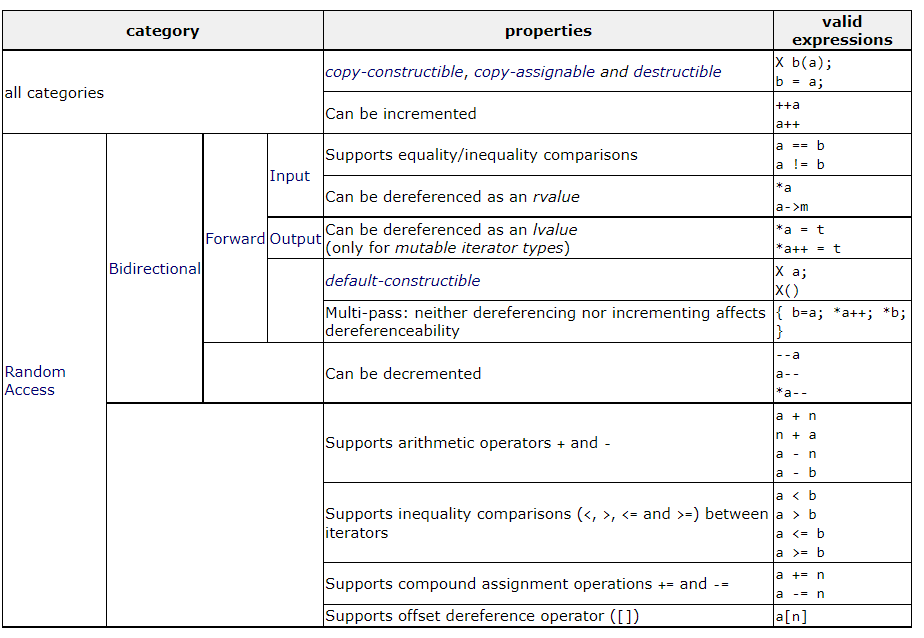
\includegraphics[scale = 0.9]{iterator.png}
\caption{Tính chất của các loại iterators}
\end{figure}
Các hàm thao tác thường dùng trên iterator:
\begin{itemize}
    \item \lstinline{next(it, steps)}: tăng biến lặp lên phía trước \lstinline{steps} lần, nếu không không có giá trị \lstinline{steps} thì hàm mặc định sẽ tăng 1, trả về \lstinline{it} sau khi đã tăng.
    \item \lstinline{prev(it, steps)}: giảm biến lặp về phía sau \lstinline{steps} lần, nếu không có giá trị \lstinline{steps} thì hàm mặc định sẽ giảm 1, trả về \lstinline{it} sau khi đã giảm.
\end{itemize}

\subsection{Containers}
\label{contain}
Một container (tạm dịch: thư viện lưu trữ) là một đối tượng lưu trữ một tập các đối tượng khác, được gọi là các phần tử của container đó. Container thường được xây dựng như các "khuôn lớp" (class template).\\
Các thư viện về “Container" (nằm trong thư viện Template chuẩn - STL) là tập hợp những lớp template và thuật toán, cho phép người lập trình có thể dễ dàng triển khai những cấu trúc dữ liệu như hàng đợi (queue),  ngăn xếp (stack), …\\
Container sẽ “sở hữu" các phần tử, tức là vòng đời của phần tử không thể vượt quá vòng đời của chính container chứa nó.\\
Có một vài cách tiếp cận về việc phân loại các containers, như trong \cite{tdtfit} chia containers thành $3$ nhóm. Ở đây chúng em sẽ chọn cách chia như trong \cite{container}, containers được chia thành $4$ nhóm:
\begin{itemize}
    \item Sequence containers: lưu trữ các phần tử theo thứ tự giống với thứ tự chúng được đưa vào container, bằng một cách thức tuyến tính (a linear manner). Nhóm này gồm \lstinline{array}, \lstinline{vector}, \lstinline{list}, \lstinline{forward_list}, và \lstinline{deque}.
    \item Container adapters: các lớp container thuộc nhóm này thực chất chỉ là các "lớp bao bọc" (wrappers) của các lớp sequence containers. Những container adapters đóng gói (encapsulate) kiểu container được bao bọc, và giới hạn user intefaces của chúng. Nhóm này gồm \lstinline{stack}, \lstinline{queue} và \lstinline{priority_queue}.
    \item Associative containers: cung cấp các cấu trúc dữ liệu được lưu trữ tự động theo một thứ tự nào đó, cho phép các thao tác tìm kiếm với độ phức tạp $O \left( {\log n} \right).$ Nhóm này thường gồm \lstinline{set}, \lstinline{map}, \lstinline{multiset}, và \lstinline{multimap}, ngoài ra còn có thể có \lstinline{hash_set}, \lstinline{hash_multiset}, \lstinline{hash_map}, \lstinline{hash_multimap}. \cite{tdtfit}
    \item Unordered associative containers: cung cấp các cấu trúc dữ liệu chưa được sắp xếp sẵn, có thể được truy cập bằng hash. Thao tác truy cập có độ phức tạp thời gian là $O \left( n \right)$ trong trường hợp xấu nhất, nhưng phần lớn phép tính có độ phức tạp tốt hơn nhiều so với độ phức tạp tuyến tính. \cite{container} Nhóm này gồm: \lstinline{unordered_set}, \lstinline{unordered_map}, \lstinline{unordered_multiset}, \lstinline{unordered_multimap}.
\end{itemize}
Mỗi container thường có một vài iterators và functions đi kèm, phục vụ cho các thao tác trên container đó. Hình \ref{popite} là các iterators thường gặp:
\begin{figure}[H]
    \centering
    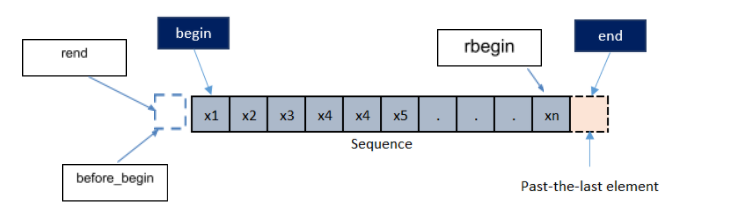
\includegraphics[scale = 1]{popite.png}
    \caption{Các iterators thường gặp}
    \label{popite}
\end{figure}
Ngoài ra, các hàm thành viên trên sẽ đi kèm với các hàm có tiền tố c- để chỉ rằng hàm trả về biến lặp hằng (const iterator) (ví dụ \lstinline{cbegin()}, \lstinline{cend()}).\\
Trong khuôn khổ báo cáo này, các loại containers sẽ được tìm hiểu cùng với iterators đi kèm.\\
Sau đây chúng ta sẽ đến với từng loại containers.